\chapter{Choosing the NoSQL Database}
\label{chap:databases}
One of the main goals of this project was to test whether connecting the 
file catalog, more specifically its metadata part, to a NoSQL database would 
improve the feedback speed of the service thus making it more pleasant to use
or make it easier to implement and maintain. The new database had to satisfy the
following conditions in order to be connectable to DIRAC and deployable in
the computing centers

\begin{itemize}
\item a freeware version has to be available for DIRAC,
\item the database has to have a python interface or client so it would be easy
to incorporate into the DIRACs code.
\end{itemize}

The characteristics of the data itself add some restrictions. The database should be
optimized for search speed. When combined with the current metadata implementation, we
get two different types of data retrieval. For directories 
the database has to be able to get all the metadata associated with a directory
identified by an ID. On the contrary, the files are fetched based on the terms in the metaquery so
all the querying techniques the metaquery could use have to be possible, including
range queries. 

%\begin{figure}[h]
%\centering
%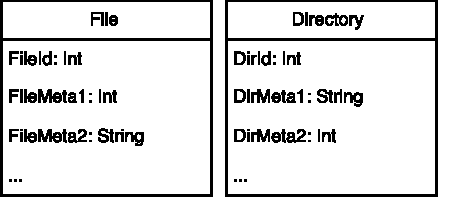
\includegraphics[scale=0.9]{dataTyp.pdf}
%\label{fig:theoDataScheme}
%\caption{Theoretical data scheme in the metadata catalog}
%\end{figure}


\section{Apache Cassandra}
Apache Cassandra\footnote{\url{http://cassandra.apache.org/}} is a distributed database for managing large amounts 
of structured data across many commodity servers, while providing highly available service and no single point 
of failure~\cite{cassandra}. Cassandra's data model is a
partitioned row store, rows are organized into tables. Each row
has an altering number of columns identified by a unique ID, which are essentially a
key-value pair. Adding that Cassandra features
its own query language CQL (Cassandra Query Language) which resembles the standard SQL 
used by all relational databases, it seems to be a perfect candidate for the metadata catalog.

\subsection{Developing a Data Model for Cassandra}

\begin{table}[t]
\parbox{.45\linewidth}{
\begin{tabular}{|l|l|l|ll}
\cline{1-4}
\multirow{2}{*}{1} & Meta1 & Meta2   & \multicolumn{1}{l|}{Meta3} &                             \\ \cline{2-4}
                   & 123   & 'alpha' & \multicolumn{1}{l|}{0}     &                             \\ \hline
\multirow{2}{*}{2} & Meta1 & Meta2   & \multicolumn{1}{l|}{Meta3} & \multicolumn{1}{l|}{Meta4}  \\ \cline{2-5} 
                   & 4000  & 'delta' & \multicolumn{1}{l|}{0}     & \multicolumn{1}{l|}{'beta'} \\ \hline
\multirow{2}{*}{3} & Meta1 & Meta3   &                            &                             \\ \cline{2-3}
                   & 200   & 1       &                            &                             \\ \cline{1-3}
\end{tabular}
\caption{First data model using Cassandra. The FileID is in the first column (row key), the next columns are metanames and their 
values.}
\label{tab:Cass1}
}
\hfill
\parbox{.45\linewidth}{
\centering
\begin{tabular}{|l|l|ll}
\hline
\multirow{2}{*}{Meta1} & 123     & \multicolumn{1}{l|}{200}     & \multicolumn{1}{l|}{4000}  \\ \cline{2-4} 
                       & \{1\}   & \multicolumn{1}{l|}{\{3\}}   & \multicolumn{1}{l|}{\{2\}} \\ \hline
\multirow{2}{*}{Meta2} & 'alpha' & \multicolumn{1}{l|}{'delta'} &                            \\ \cline{2-3}
                       & \{1\}   & \multicolumn{1}{l|}{\{2\}}   &                            \\ \cline{1-3}
\multirow{2}{*}{Meta3} & 0       & \multicolumn{1}{l|}{1}       &                            \\ \cline{2-3}
                       & \{1,2\} & \multicolumn{1}{l|}{\{3\}}   &                            \\ \cline{1-3}
\multirow{2}{*}{Meta4} & 'beta'  &                              &                            \\ \cline{2-2}
                       & \{2\}   &                              &                            \\ \cline{1-2}
\end{tabular}
\caption{Second Cassandra scheme. FileIDs are now in sets in column values, metanames are row keys and metavalues are columns names.}
\label{tab:fileMeta}
}
\end{table}

Although CQL makes it look like a relational database, the developer has to keep in mind that
Cassandra is different. Our first scheme used the altering number of columns and organized the 
data in tables, where each file or directory had its own row with metanames as column
names and values as column values (see Table~\ref{tab:Cass1}).
%(this model strongly resembles the theoretical data scheme in Figure~\ref{fig:theoDataScheme}). 
Secondary indices were created over column values so that 
the query would be possible. Although CQLs' similarity with SQL would suggest otherwise, 
it turned out that this kind of indexing does not support range queries so this data-model
had to be abandoned. 

After understanding more thoroughly how Cassandra works, another data-model was introduced 
utilizing most of Cassandra specific features. The key properties Cassandra guaranties are that 
rows are not divided across multiple nodes in the cluster and column keys inside the row
are sorted. Based on these two characteristics a functioning data model was created. For  
directories row IDs are mapped on directory IDs and the model the same as the previous one. 
Retrieving a row with a given row ID is one of the supported operations.
For files each metaname has its row, column names are meta values and column values are sets of 
fileIDs of files having this metaname and value associated with them (see Table~\ref{tab:fileMeta}). 

%\begin{table}[t]
%\centering
%\begin{tabular}{|l|l|ll}
%\hline
%\multirow{2}{*}{Meta1} & 123     & \multicolumn{1}{l|}{200}     & \multicolumn{1}{l|}{4000}  \\ \cline{2-4} 
%                       & \{1\}   & \multicolumn{1}{l|}{\{3\}}   & \multicolumn{1}{l|}{\{2\}} \\ \hline
%\multirow{2}{*}{Meta2} & 'alpha' & \multicolumn{1}{l|}{'delta'} &                            \\ \cline{2-3}
%                       & \{1\}   & \multicolumn{1}{l|}{\{2\}}   &                            \\ \cline{1-3}
%\multirow{2}{*}{Meta3} & 0       & \multicolumn{1}{l|}{1}       &                            \\ \cline{2-3}
%                       & \{1,2\} & \multicolumn{1}{l|}{\{3\}}   &                            \\ \cline{1-3}
%\multirow{2}{*}{Meta4} & 'beta'  &                              &                            \\ \cline{2-2}
%                       & \{2\}   &                              &                            \\ \cline{1-2}
%\end{tabular}
%\caption{File metadata}
%\label{tab:fileMeta}
%\end{table}

The rows are grouped in tables by value type, because the algorithm used to sort the
column names is unified per table. There is also an index over fileID sets, 
so that retrieving all metadata for one specific file is possible. However the scheme is 
not optimized for this operation, because this is done only for the users information and
when setting new metadata.

\begin{listing}
\begin{minted}{sql}
CREATE TABLE file_int (
    metaname text,
    value int,
    fileid set<int>,
    PRIMARY KEY (metaname, value)
);
\end{minted}
\caption{Data structure described using CQL}
\label{lis:CQLstruct}
\end{listing}

In CQL this structure looks like a table with three columns and a compound primary key (see 
Listing~\ref{lis:CQLstruct}). 
This brings the main disadvantage of this approach: meta names can be queried only one at a time and
the result has to be then finalized in the DIRACs code. The expected structure of data could
suggest that the number of files satisfying only a part of the metaquery can be large, the idea of using 
Cassandra as the File Catalog database was abandoned, because fetching multiple times a large number of 
files from the database and then doing an intersection in the python code is not optimal. 

%\begin{listing}
%\begin{minted}{sql}
%SELECT fileid 
%	FROM file_int 
%	WHERE metaname='metaInt1' AND value>3;
%\end{minted}
%\caption{Example query}
%\end{listing}


\section{Document Databases}

A document-oriented database replaces the concept of a \textit{row} from the world of relational 
databases with a more dynamic and versatile \textit{document}. By allowing arrays and embedded documents the 
document-oriented databases provide de-normalization of the data and complex 
relationships in a single document. Also there are no predefined schemes, which is essential for our project, because 
the number of associated metadata varies between 
files. The metadata are stored in simple a JSON structure with names being metanames (see Listing~\ref{lis:json}).

\begin{listing}[t]
\begin{lstlisting}
{
	'id'       : id
	'metaInt1' : 1,
	'metaStr1' : 'qwerty',
	'metaInt3' : 123
}
\end{lstlisting}
\caption{Metadata stored in a document database. This is a basic example, there can be many more fields in the JSON structure, but it will always remain a simple structure.}
\label{lis:json}
\end{listing}

Document databases were not the first choice during developing this project, because the idea of
storing metadata in a JSON structure and then building indices above the properties is not as
familiar as Cassandras columns. But it turned out to be even easier to use.

\subsection{MongoDB}

MongoDB is an open-source document-oriented database storing JSON files. Currently, in November 2015, MongoDB is the fourth 
most popular type of database management system, and the most popular for document stores~\cite{MongoPop}. 
In MongoDB the document is the basic unit, documents are grouped into collections. A single instance of MongoDB can host
multiple databases, each grouping together multiple collections. In collections documents are identified using a special 
field \texttt{\_id} which has to be unique within a collection~\cite{MongoBook}. This projects maps the file or directory 
ids from the file catalog to this id field.

\subsubsection{Using MongoDB}

On Scientific Linux it can be installed from a package so the initial set up is rather easy.
MongoDB comes with its own shell based on
JavaScript, which the administrator can use to query and update data as well as perform administrative 
operations\footnote{\url{https://docs.mongodb.org/getting-started/shell/client/}}. The client is rather easy-to-use 
and its commands are very similar to those used by the python library. The mongo
package also contains several tools for monitoring the database
including the \texttt{mongotop}\footnote{\url{https://docs.mongodb.org/manual/reference/program/mongotop/}} 
and \texttt{mongostat}\footnote{\url{https://docs.mongodb.org/manual/reference/program/mongostat/}}, and several 
other helping the administrator with e.g. dumping and restoring the database. For further 
debugging the log file provides a sufficient amount of information, when its verbosity is turned up to at least 3.
Overall the database is easy to use and administer thanks to many well documented utilities. 

There are two types
of configuration files supported by MongoDB: the older one in form of \texttt{<setting> = <value>} and the 
newer using YAML format~\cite{YAML}. The database comes with the older one (although it is not developed since version 
2.4), but most of the configuration documentation is in the newer one (and some of the new features can be only set in 
YAML format) so the administrator should convert it manually before using the database since it could ease
the usage and optional re-configuration later.
The major drawback when using this database is that every property has to be indexed manually, which not only 
takes time, but also consumes disk space.

% When querying in a collection that does not exist, there is no error, just no result, which can be confusing

\subsection{Elasticsearch}

Elasticsearch (ES)\footnote{\url{https://www.elastic.co/products/elasticsearch}} is a real-time distributed open-source 
analytics and search engine~\cite{ESBook} 
built on top of Apache Lucene\footnote{\url{https://lucene.apache.org/}}. Unlike very complex Lucene, 
ES features a simple RESTful API that makes it easy to use. Moreover it can be used not only 
for full-text search, but also for real-time analytics or, which is important for this project, as a 
distributed document store, where \textit{every} field is indexed and searchable. Its python 
client\footnote{\url{http://elasticsearch-py.readthedocs.org/en/master/}} provides a wrapper for the RESTful API
as well as some useful additional commands called helpers (e.g. for bulk loading data, the command 
\texttt{helpers.bulk(es, dataToLoad(size))} was used).

\subsubsection{Using ES}

Like MongoDB, Elasticsearch comes in a package. The installation set reasonable 
defaults (the only thing that was changed on the testing server was the data directory and listening on the 
universal IP address had to be enabled, because the default is only local host). The 
configuration file is in YAML format. There is no need for any initial data structure,
the first data is simply inserted using the correct URL\footnote{\url{http://host:port/index/doc_type/doc_id}
is the URL the RESTful API uses, when using the python library \texttt{index, doc\_type}\texttt{doc\_id} are 
specified using the function arguments}. In ES, a document belongs to a type and types are contained by indices 
(hence the \texttt{index} and \texttt{doc\_type} in the command). 
An Elasticsearch cluster can contain multiple indices, which can contain 
multiple types (there is a rough parallel with the world of relational databases, where indices would be databases 
and types would correspond to tables). Unlike the relational databases ES can create the index and type with the 
first inserted document using its default configuration.

% When a value of a field is set to a non-numeric value, a numeric_range query cannot be executed after that, even though all the currently set values are numeric

\section{Database Tests}

For testing, a single IBM iDataPlex dx340 server was used, equipped with 2x Intel Xeon 5440 with 4 cores, 16GB
of RAM and 300GB SAS hard disk, where all the database files were stored. After several smaller datasets, 
the main testing data was generated trying to mimic the DIRAC production data structure. There is expected 
over 10 million files with approximately 20 different meta names.
The generated set had $(10 000 000 - 1)$ files with $1$ to $998$ metanames associated with them\footnote{ 
The generator chose a randomly $1$ to $499$ integer metrics and the same number of string ones.}, which is more
than the production data would have, but gave the testing more data to encumber the databases.
The metrics names were \texttt{test[Int|Str]NNN}, where \texttt{NNN} stands for a number. The
integer values were all picked from the interval $[1;1000]$ and the string values were one of the
words from the NATO phonetic alphabet~\cite{NATO}, which lead to easier composition of testing queries. 
Integer fields represent continuous data types and string fields represent discreet data types.

The data was stored in two CSV files with lines \texttt{id,metaname,value} and the sizes of 53 and 59~GB.

\subsection{Loading the Big Data}

Both databases feature bulk loading functionality. Although the user will not probably use it, in
this project, which involved testing the databases on a large data, the loading of the them was one 
of the challenges.

ES python interface features a bulk load function (the default data chunk size is 500 records). 
Unfortunately it crashes on a TimeoutException from time to time, making the loading by a simple script a rather long 
procedure. We have not been able to discover the cause of the exception.

MongoDB features a command \texttt{mongoimport} which can read a file of JSON objects and load
them all. Its pace on the test data was approximately $150-200$ entries per second. Unfortunately 
the script froze from time to time so loading the whole dataset took again several days. Once the data was
loaded, it could be backed up using the utility \texttt{mongodump} and then again loaded using the 
command \texttt{mongorestore}. These two utilities ran without problems and were used when changing the 
storage engine.

\subsection{Testing Query Performance on a Predefined Sample}

The task of the database in this deployment will be to accept a query, execute the search and return all the 
ids of documents\footnote{Document ids are mapped on file ids, so this procedure is returning the ids of files
that satisfy the query} satisfying the query. To measure the results as precisely as possible, a list of
queries was generated. When testing one database, all other database services were stopped so that they did not
interfere with the test. As we mentioned, to effectively search for data in MongoDB the document properties have to be 
indexed manually. Indices were made on several integer fields (testInt1-8) and three string fields 
(testStr1,testStr2,testStr3). The time cost of building\footnote{for the default storage engine} the 
indices and their space requirements are listed in Table~\ref{tab:indexBuildTimes}.

\begin{table}[h]
\centering
\begin{tabular}{lcccc}
\toprule
\textbf{Field}   & & \textbf{Time}     & \textbf{Disk Space (MMAP)} & \textbf{Disk Space (WT)} \\ \midrule
testInt1 & & 00:20:50 & 211 390           & 46 785          \\ \hline
testInt2 & & 00:20:00 & 211 407           & 46 789          \\ \hline
testInt3 & & 00:19:59 & 211 390           & 46 785          \\ \hline
testInt4 & & 00:20:12 & 211 415           & 46 789          \\ \hline
testInt5 & & 00:19:58 & 211 390           & 46 785          \\ \hline
testStr1 & & 00:20:06 & 203 043           & 44 351          \\ \hline
testStr2 & & 00:20:13 & 203 026           & 44 351          \\ \hline
testStr3 & & 00:20:51 & 203 043           & 44 356          \\ \hline
testInt6 & & 00:21:03 & 211 407           & 46 789          \\ \hline
testInt7 & & 00:19:57 & 211 399           & 46 785          \\ \hline
testInt8 & & 00:19:58 & 211 390           & 46 785          \\ \toprule
\end{tabular}
\caption{The time and storage requirements for indices used in MongoDB. The indices were built while using
the MMAP storage engine. Sizes are in MB.}
\label{tab:indexBuildTimes}
\end{table}

ES does not have a similar limitation, however the queries were kept
the same so that the comparison is as correct as possible.

The queries were generated randomly combining the integer and string properties. The number of hits was not 
considered while generating the queries. All the queries used can be found in Appendix~\ref{app:queries}.

The program testing the performance is a python script running on a personal computer in the same LAN as the 
database machine (similarly to the expected deployment of the service). The measured time is the interval between 
the moment the query was submitted, to the moment the results were extracted to a python list. Neither the 
preparation of the query, nor the printing of the results were included in the final time. 

For ES the cache of the index was flushed after every query to keep the results consistent (although as 
Figure~\ref{fig:EScache} suggests, flushing the cache does not make a notable difference for bigger data volumes). 

\begin{figure}[h]
	\centering
	% GNUPLOT: LaTeX picture with Postscript
\begingroup
  \makeatletter
  \providecommand\color[2][]{%
    \GenericError{(gnuplot) \space\space\space\@spaces}{%
      Package color not loaded in conjunction with
      terminal option `colourtext'%
    }{See the gnuplot documentation for explanation.%
    }{Either use 'blacktext' in gnuplot or load the package
      color.sty in LaTeX.}%
    \renewcommand\color[2][]{}%
  }%
  \providecommand\includegraphics[2][]{%
    \GenericError{(gnuplot) \space\space\space\@spaces}{%
      Package graphicx or graphics not loaded%
    }{See the gnuplot documentation for explanation.%
    }{The gnuplot epslatex terminal needs graphicx.sty or graphics.sty.}%
    \renewcommand\includegraphics[2][]{}%
  }%
  \providecommand\rotatebox[2]{#2}%
  \@ifundefined{ifGPcolor}{%
    \newif\ifGPcolor
    \GPcolortrue
  }{}%
  \@ifundefined{ifGPblacktext}{%
    \newif\ifGPblacktext
    \GPblacktextfalse
  }{}%
  % define a \g@addto@macro without @ in the name:
  \let\gplgaddtomacro\g@addto@macro
  % define empty templates for all commands taking text:
  \gdef\gplbacktext{}%
  \gdef\gplfronttext{}%
  \makeatother
  \ifGPblacktext
    % no textcolor at all
    \def\colorrgb#1{}%
    \def\colorgray#1{}%
  \else
    % gray or color?
    \ifGPcolor
      \def\colorrgb#1{\color[rgb]{#1}}%
      \def\colorgray#1{\color[gray]{#1}}%
      \expandafter\def\csname LTw\endcsname{\color{white}}%
      \expandafter\def\csname LTb\endcsname{\color{black}}%
      \expandafter\def\csname LTa\endcsname{\color{black}}%
      \expandafter\def\csname LT0\endcsname{\color[rgb]{1,0,0}}%
      \expandafter\def\csname LT1\endcsname{\color[rgb]{0,1,0}}%
      \expandafter\def\csname LT2\endcsname{\color[rgb]{0,0,1}}%
      \expandafter\def\csname LT3\endcsname{\color[rgb]{1,0,1}}%
      \expandafter\def\csname LT4\endcsname{\color[rgb]{0,1,1}}%
      \expandafter\def\csname LT5\endcsname{\color[rgb]{1,1,0}}%
      \expandafter\def\csname LT6\endcsname{\color[rgb]{0,0,0}}%
      \expandafter\def\csname LT7\endcsname{\color[rgb]{1,0.3,0}}%
      \expandafter\def\csname LT8\endcsname{\color[rgb]{0.5,0.5,0.5}}%
    \else
      % gray
      \def\colorrgb#1{\color{black}}%
      \def\colorgray#1{\color[gray]{#1}}%
      \expandafter\def\csname LTw\endcsname{\color{white}}%
      \expandafter\def\csname LTb\endcsname{\color{black}}%
      \expandafter\def\csname LTa\endcsname{\color{black}}%
      \expandafter\def\csname LT0\endcsname{\color{black}}%
      \expandafter\def\csname LT1\endcsname{\color{black}}%
      \expandafter\def\csname LT2\endcsname{\color{black}}%
      \expandafter\def\csname LT3\endcsname{\color{black}}%
      \expandafter\def\csname LT4\endcsname{\color{black}}%
      \expandafter\def\csname LT5\endcsname{\color{black}}%
      \expandafter\def\csname LT6\endcsname{\color{black}}%
      \expandafter\def\csname LT7\endcsname{\color{black}}%
      \expandafter\def\csname LT8\endcsname{\color{black}}%
    \fi
  \fi
  \setlength{\unitlength}{0.0500bp}%
  \begin{picture}(8502.00,3968.00)%
    \gplgaddtomacro\gplbacktext{%
      \csname LTb\endcsname%
      \put(1210,440){\makebox(0,0)[r]{\strut{} 0.01}}%
      \put(1210,874){\makebox(0,0)[r]{\strut{} 0.1}}%
      \put(1210,1308){\makebox(0,0)[r]{\strut{} 1}}%
      \put(1210,1741){\makebox(0,0)[r]{\strut{} 10}}%
      \put(1210,2175){\makebox(0,0)[r]{\strut{} 100}}%
      \put(1210,2609){\makebox(0,0)[r]{\strut{} 1000}}%
      \put(1210,3043){\makebox(0,0)[r]{\strut{} 10000}}%
      \put(1342,220){\makebox(0,0){\strut{} 0}}%
      \put(2153,220){\makebox(0,0){\strut{} 5}}%
      \put(2965,220){\makebox(0,0){\strut{} 10}}%
      \put(3776,220){\makebox(0,0){\strut{} 15}}%
      \put(4587,220){\makebox(0,0){\strut{} 20}}%
      \put(5399,220){\makebox(0,0){\strut{} 25}}%
      \put(6210,220){\makebox(0,0){\strut{} 30}}%
      \put(6829,440){\makebox(0,0)[l]{\strut{} 1}}%
      \put(6829,812){\makebox(0,0)[l]{\strut{} 10}}%
      \put(6829,1184){\makebox(0,0)[l]{\strut{} 100}}%
      \put(6829,1556){\makebox(0,0)[l]{\strut{} 1000}}%
      \put(6829,1927){\makebox(0,0)[l]{\strut{} 10000}}%
      \put(6829,2299){\makebox(0,0)[l]{\strut{} 100000}}%
      \put(6829,2671){\makebox(0,0)[l]{\strut{} 1e+06}}%
      \put(6829,3043){\makebox(0,0)[l]{\strut{} 1e+07}}%
      \put(176,1741){\rotatebox{-270}{\makebox(0,0){\strut{}time(s)}}}%
      \put(7994,1741){\rotatebox{-270}{\makebox(0,0){\strut{}number of hits}}}%
    }%
    \gplgaddtomacro\gplfronttext{%
      \csname LTb\endcsname%
      \put(3164,3795){\makebox(0,0)[r]{\strut{}number of hits}}%
      \csname LTb\endcsname%
      \put(3164,3575){\makebox(0,0)[r]{\strut{}ES without cache (s)}}%
      \csname LTb\endcsname%
      \put(6659,3795){\makebox(0,0)[r]{\strut{}ES (s)}}%
    }%
    \gplbacktext
    \put(0,0){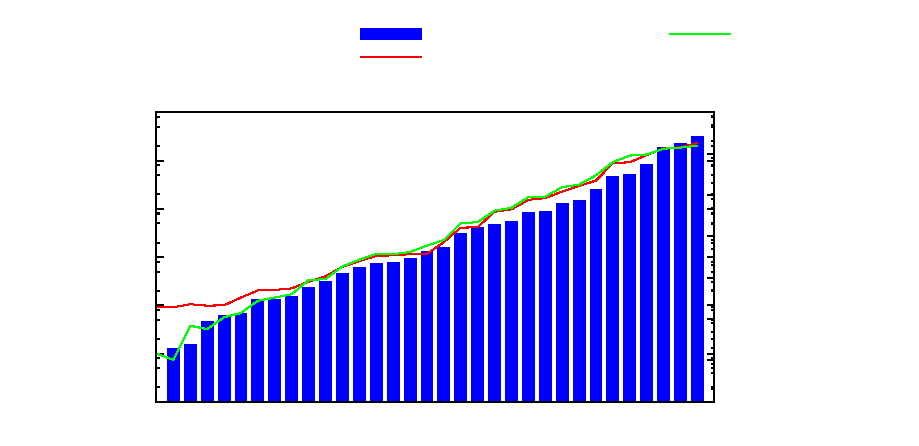
\includegraphics{ES_comparison2}}%
    \gplfronttext
  \end{picture}%
\endgroup

%	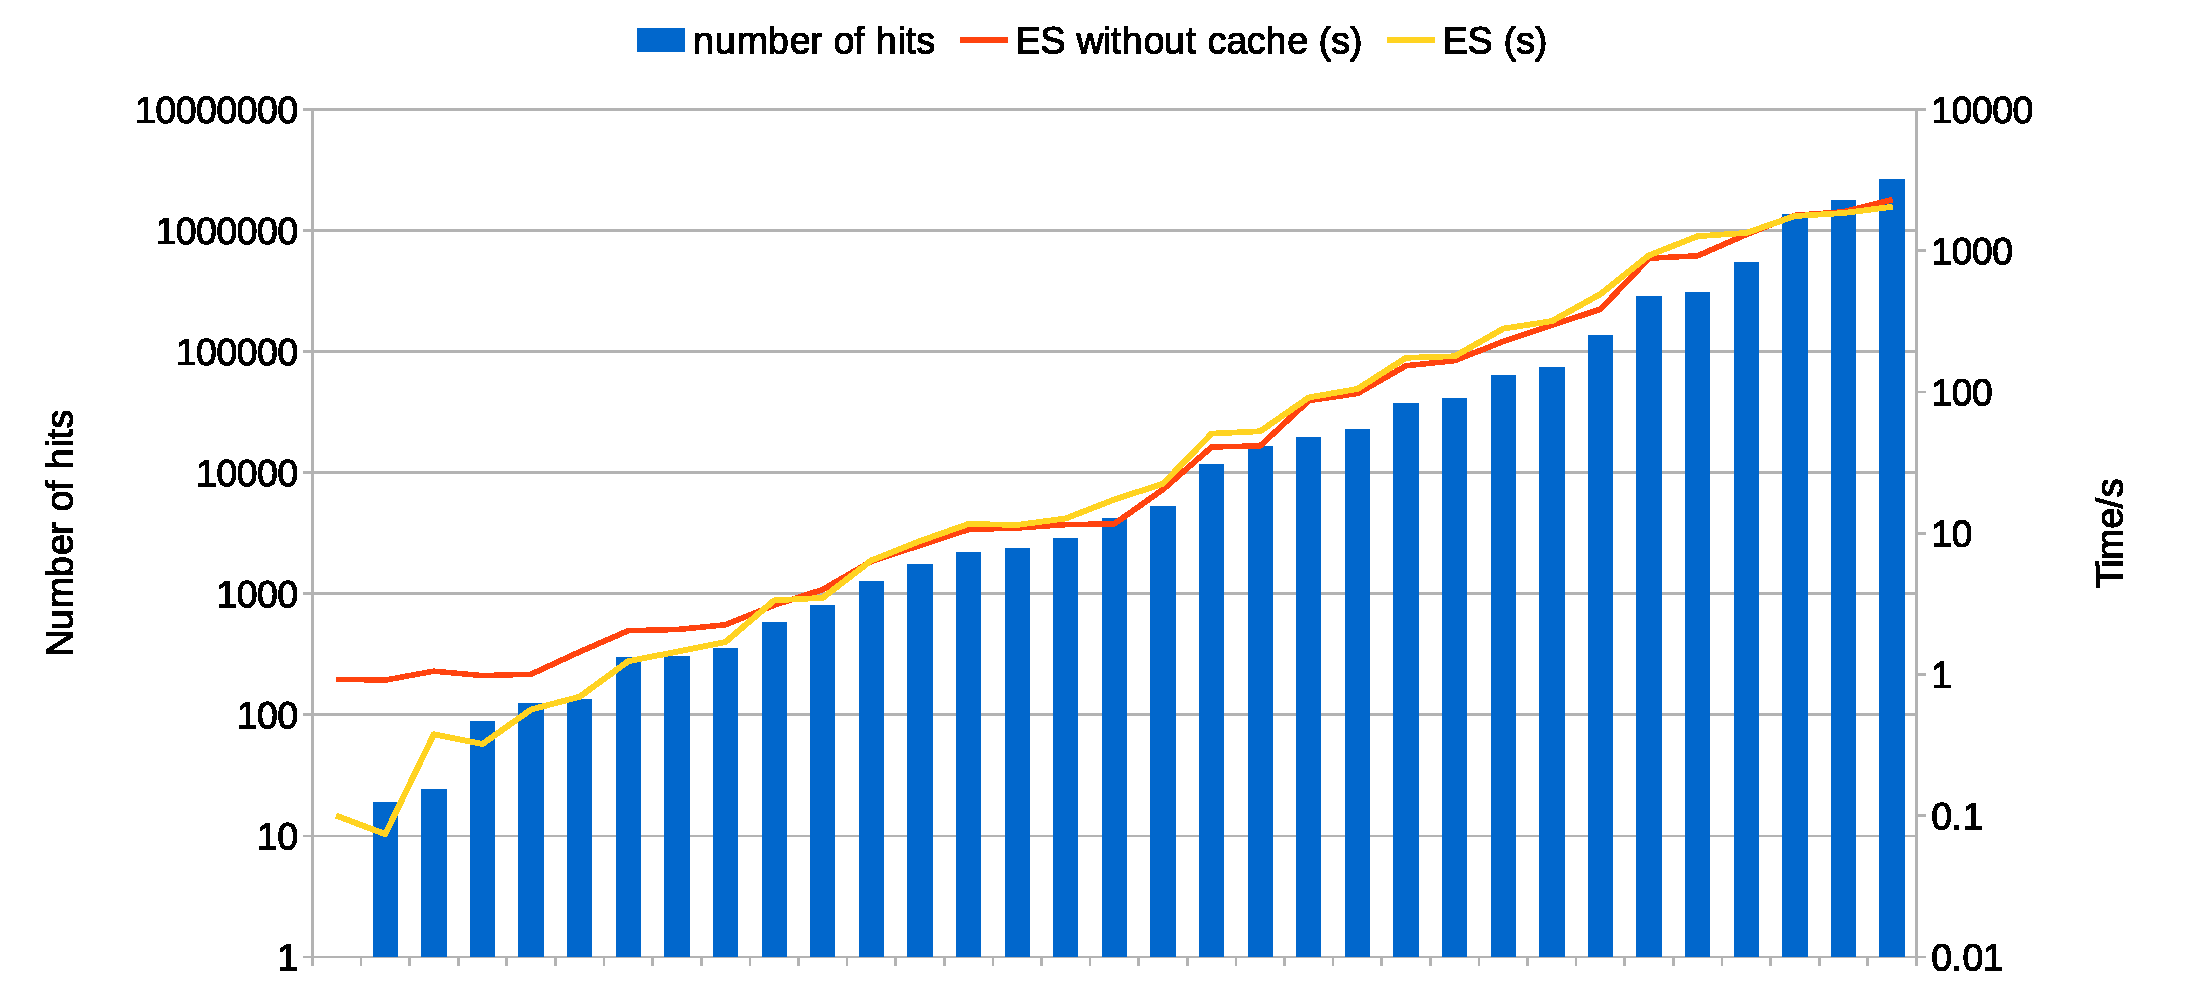
\includegraphics[width=\textwidth]{ES_comparison.pdf}
	\caption{Query times for Elasticsearch comparing performance with and without dumping depending on the number of 
	hits (logarithmic scale)}
	\label{fig:EScache}
\end{figure}
\pagebreak
The original MongoDB instance was using the default storage engine used by versions up to 3.0\footnote{MMAPv1 
Storage Engine based on memory mapped files}. There is also a new storage engine WiredTiger\footnote{
\url{https://docs.mongodb.org/manual/core/wiredtiger/}} available and their performances were compared.
Moreover the new engine brings the option of choosing the compression strategy. The comparison of disk space usage 
can be seen in Table~\ref{tab:MongoComp} and query performance in Figure~\ref{fig:MDBcomparison}.

\begin{table}[t]
\centering
\begin{tabular}{lccc}
\toprule
\textbf{Storage Engine}       & \textbf{Total Database Size} & \textbf{Total Index Size} \\ 
\midrule
MMAPv1                        & 136 161                      & 2 579 \\ 
WiredTiger with zlib comp.    & 22 788                       & 615   \\ 
WiredTiger with default comp. & 42 249                       & 616   \\ 
\toprule
\end{tabular}
\caption{Disk usage comparison of MongoDBs storage engines. Note the size of the indices does not depend on the
compression used. All sizes are in MB.}
\label{tab:MongoComp}
\end{table}

\begin{figure}[h]
	\centering
	% GNUPLOT: LaTeX picture with Postscript
\begingroup
  \makeatletter
  \providecommand\color[2][]{%
    \GenericError{(gnuplot) \space\space\space\@spaces}{%
      Package color not loaded in conjunction with
      terminal option `colourtext'%
    }{See the gnuplot documentation for explanation.%
    }{Either use 'blacktext' in gnuplot or load the package
      color.sty in LaTeX.}%
    \renewcommand\color[2][]{}%
  }%
  \providecommand\includegraphics[2][]{%
    \GenericError{(gnuplot) \space\space\space\@spaces}{%
      Package graphicx or graphics not loaded%
    }{See the gnuplot documentation for explanation.%
    }{The gnuplot epslatex terminal needs graphicx.sty or graphics.sty.}%
    \renewcommand\includegraphics[2][]{}%
  }%
  \providecommand\rotatebox[2]{#2}%
  \@ifundefined{ifGPcolor}{%
    \newif\ifGPcolor
    \GPcolortrue
  }{}%
  \@ifundefined{ifGPblacktext}{%
    \newif\ifGPblacktext
    \GPblacktextfalse
  }{}%
  % define a \g@addto@macro without @ in the name:
  \let\gplgaddtomacro\g@addto@macro
  % define empty templates for all commands taking text:
  \gdef\gplbacktext{}%
  \gdef\gplfronttext{}%
  \makeatother
  \ifGPblacktext
    % no textcolor at all
    \def\colorrgb#1{}%
    \def\colorgray#1{}%
  \else
    % gray or color?
    \ifGPcolor
      \def\colorrgb#1{\color[rgb]{#1}}%
      \def\colorgray#1{\color[gray]{#1}}%
      \expandafter\def\csname LTw\endcsname{\color{white}}%
      \expandafter\def\csname LTb\endcsname{\color{black}}%
      \expandafter\def\csname LTa\endcsname{\color{black}}%
      \expandafter\def\csname LT0\endcsname{\color[rgb]{1,0,0}}%
      \expandafter\def\csname LT1\endcsname{\color[rgb]{0,1,0}}%
      \expandafter\def\csname LT2\endcsname{\color[rgb]{0,0,1}}%
      \expandafter\def\csname LT3\endcsname{\color[rgb]{1,0,1}}%
      \expandafter\def\csname LT4\endcsname{\color[rgb]{0,1,1}}%
      \expandafter\def\csname LT5\endcsname{\color[rgb]{1,1,0}}%
      \expandafter\def\csname LT6\endcsname{\color[rgb]{0,0,0}}%
      \expandafter\def\csname LT7\endcsname{\color[rgb]{1,0.3,0}}%
      \expandafter\def\csname LT8\endcsname{\color[rgb]{0.5,0.5,0.5}}%
    \else
      % gray
      \def\colorrgb#1{\color{black}}%
      \def\colorgray#1{\color[gray]{#1}}%
      \expandafter\def\csname LTw\endcsname{\color{white}}%
      \expandafter\def\csname LTb\endcsname{\color{black}}%
      \expandafter\def\csname LTa\endcsname{\color{black}}%
      \expandafter\def\csname LT0\endcsname{\color{black}}%
      \expandafter\def\csname LT1\endcsname{\color{black}}%
      \expandafter\def\csname LT2\endcsname{\color{black}}%
      \expandafter\def\csname LT3\endcsname{\color{black}}%
      \expandafter\def\csname LT4\endcsname{\color{black}}%
      \expandafter\def\csname LT5\endcsname{\color{black}}%
      \expandafter\def\csname LT6\endcsname{\color{black}}%
      \expandafter\def\csname LT7\endcsname{\color{black}}%
      \expandafter\def\csname LT8\endcsname{\color{black}}%
    \fi
  \fi
  \setlength{\unitlength}{0.0500bp}%
  \begin{picture}(8502.00,3968.00)%
    \gplgaddtomacro\gplbacktext{%
      \csname LTb\endcsname%
      \put(1342,440){\makebox(0,0)[r]{\strut{} 0.01}}%
      \put(1342,812){\makebox(0,0)[r]{\strut{} 0.1}}%
      \put(1342,1184){\makebox(0,0)[r]{\strut{} 1}}%
      \put(1342,1556){\makebox(0,0)[r]{\strut{} 10}}%
      \put(1342,1927){\makebox(0,0)[r]{\strut{} 100}}%
      \put(1342,2299){\makebox(0,0)[r]{\strut{} 1000}}%
      \put(1342,2671){\makebox(0,0)[r]{\strut{} 10000}}%
      \put(1342,3043){\makebox(0,0)[r]{\strut{} 100000}}%
      \put(1474,220){\makebox(0,0){\strut{} 0}}%
      \put(2265,220){\makebox(0,0){\strut{} 5}}%
      \put(3057,220){\makebox(0,0){\strut{} 10}}%
      \put(3848,220){\makebox(0,0){\strut{} 15}}%
      \put(4639,220){\makebox(0,0){\strut{} 20}}%
      \put(5431,220){\makebox(0,0){\strut{} 25}}%
      \put(6222,220){\makebox(0,0){\strut{} 30}}%
      \put(6829,440){\makebox(0,0)[l]{\strut{} 1}}%
      \put(6829,812){\makebox(0,0)[l]{\strut{} 10}}%
      \put(6829,1184){\makebox(0,0)[l]{\strut{} 100}}%
      \put(6829,1556){\makebox(0,0)[l]{\strut{} 1000}}%
      \put(6829,1927){\makebox(0,0)[l]{\strut{} 10000}}%
      \put(6829,2299){\makebox(0,0)[l]{\strut{} 100000}}%
      \put(6829,2671){\makebox(0,0)[l]{\strut{} 1e+06}}%
      \put(6829,3043){\makebox(0,0)[l]{\strut{} 1e+07}}%
      \put(176,1741){\rotatebox{-270}{\makebox(0,0){\strut{}time(s)}}}%
      \put(7994,1741){\rotatebox{-270}{\makebox(0,0){\strut{}number of hits}}}%
    }%
    \gplgaddtomacro\gplfronttext{%
      \csname LTb\endcsname%
      \put(3230,3795){\makebox(0,0)[r]{\strut{}number of hits}}%
      \csname LTb\endcsname%
      \put(3230,3575){\makebox(0,0)[r]{\strut{}MDB}}%
      \csname LTb\endcsname%
      \put(5933,3795){\makebox(0,0)[r]{\strut{}MDB WT zlib}}%
      \csname LTb\endcsname%
      \put(5933,3575){\makebox(0,0)[r]{\strut{}MDB WT}}%
    }%
    \gplbacktext
    \put(0,0){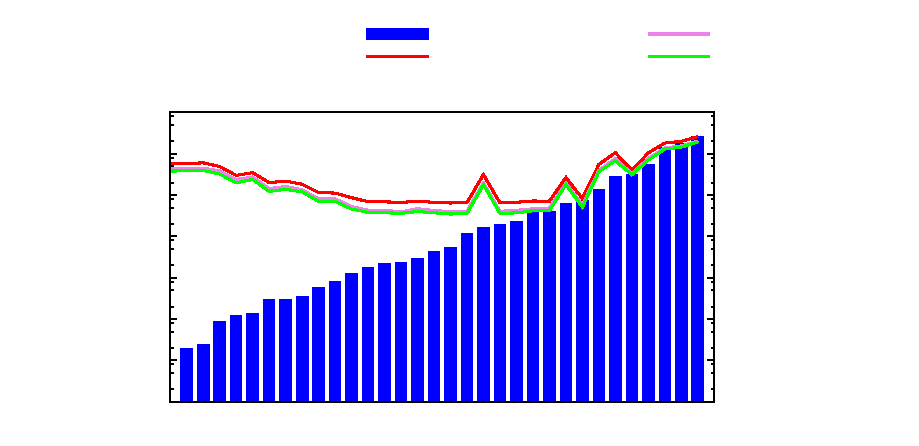
\includegraphics{MDB_comparison2}}%
    \gplfronttext
  \end{picture}%
\endgroup

	%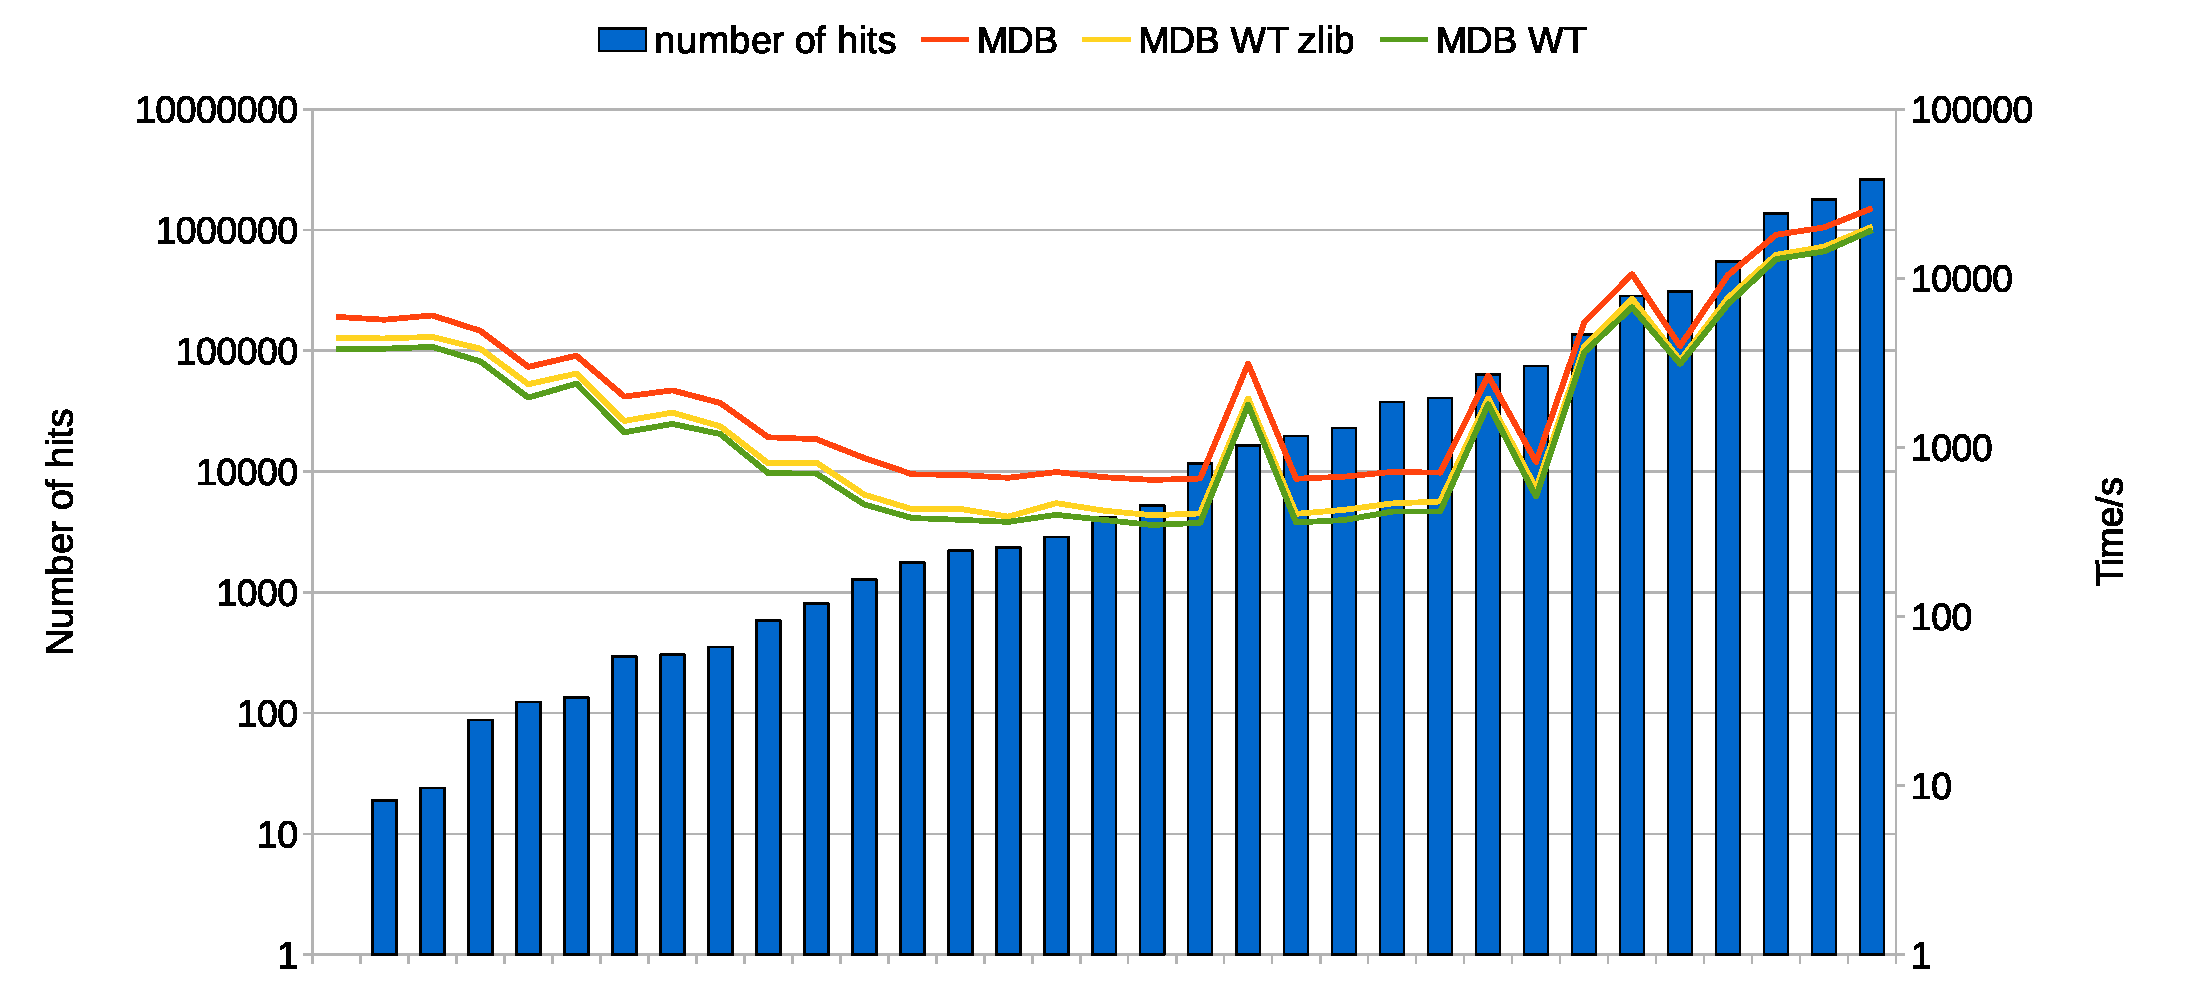
\includegraphics[width=\textwidth]{MDB_comparison.pdf}
	\caption{Query times for MongoDB comparing performance with different storage engines and compression 
	options: the old MMAPv1 (MDB), the newly available WiredTiger (MDB WT) and WiredTiger with extra compression 
	(MDB WT zlib). Logarithmic scale.}
	\label{fig:MDBcomparison}
\end{figure}

We can conclude as follows: if the administrator does not have a critically low amount of disk space available, MongoDB
works best with the new WiredTiger storage engine with the default compression. In Figure~\ref{fig:DBscomparison} we 
can see the comparison of performance on the sample queries between the WiredTiger configuration of MongoDB and 
Elasticsearch. 

\begin{figure}[h]
	\centering
	% GNUPLOT: LaTeX picture with Postscript
\begingroup
  \makeatletter
  \providecommand\color[2][]{%
    \GenericError{(gnuplot) \space\space\space\@spaces}{%
      Package color not loaded in conjunction with
      terminal option `colourtext'%
    }{See the gnuplot documentation for explanation.%
    }{Either use 'blacktext' in gnuplot or load the package
      color.sty in LaTeX.}%
    \renewcommand\color[2][]{}%
  }%
  \providecommand\includegraphics[2][]{%
    \GenericError{(gnuplot) \space\space\space\@spaces}{%
      Package graphicx or graphics not loaded%
    }{See the gnuplot documentation for explanation.%
    }{The gnuplot epslatex terminal needs graphicx.sty or graphics.sty.}%
    \renewcommand\includegraphics[2][]{}%
  }%
  \providecommand\rotatebox[2]{#2}%
  \@ifundefined{ifGPcolor}{%
    \newif\ifGPcolor
    \GPcolortrue
  }{}%
  \@ifundefined{ifGPblacktext}{%
    \newif\ifGPblacktext
    \GPblacktextfalse
  }{}%
  % define a \g@addto@macro without @ in the name:
  \let\gplgaddtomacro\g@addto@macro
  % define empty templates for all commands taking text:
  \gdef\gplbacktext{}%
  \gdef\gplfronttext{}%
  \makeatother
  \ifGPblacktext
    % no textcolor at all
    \def\colorrgb#1{}%
    \def\colorgray#1{}%
  \else
    % gray or color?
    \ifGPcolor
      \def\colorrgb#1{\color[rgb]{#1}}%
      \def\colorgray#1{\color[gray]{#1}}%
      \expandafter\def\csname LTw\endcsname{\color{white}}%
      \expandafter\def\csname LTb\endcsname{\color{black}}%
      \expandafter\def\csname LTa\endcsname{\color{black}}%
      \expandafter\def\csname LT0\endcsname{\color[rgb]{1,0,0}}%
      \expandafter\def\csname LT1\endcsname{\color[rgb]{0,1,0}}%
      \expandafter\def\csname LT2\endcsname{\color[rgb]{0,0,1}}%
      \expandafter\def\csname LT3\endcsname{\color[rgb]{1,0,1}}%
      \expandafter\def\csname LT4\endcsname{\color[rgb]{0,1,1}}%
      \expandafter\def\csname LT5\endcsname{\color[rgb]{1,1,0}}%
      \expandafter\def\csname LT6\endcsname{\color[rgb]{0,0,0}}%
      \expandafter\def\csname LT7\endcsname{\color[rgb]{1,0.3,0}}%
      \expandafter\def\csname LT8\endcsname{\color[rgb]{0.5,0.5,0.5}}%
    \else
      % gray
      \def\colorrgb#1{\color{black}}%
      \def\colorgray#1{\color[gray]{#1}}%
      \expandafter\def\csname LTw\endcsname{\color{white}}%
      \expandafter\def\csname LTb\endcsname{\color{black}}%
      \expandafter\def\csname LTa\endcsname{\color{black}}%
      \expandafter\def\csname LT0\endcsname{\color{black}}%
      \expandafter\def\csname LT1\endcsname{\color{black}}%
      \expandafter\def\csname LT2\endcsname{\color{black}}%
      \expandafter\def\csname LT3\endcsname{\color{black}}%
      \expandafter\def\csname LT4\endcsname{\color{black}}%
      \expandafter\def\csname LT5\endcsname{\color{black}}%
      \expandafter\def\csname LT6\endcsname{\color{black}}%
      \expandafter\def\csname LT7\endcsname{\color{black}}%
      \expandafter\def\csname LT8\endcsname{\color{black}}%
    \fi
  \fi
  \setlength{\unitlength}{0.0500bp}%
  \begin{picture}(8502.00,3968.00)%
    \gplgaddtomacro\gplbacktext{%
      \csname LTb\endcsname%
      \put(1210,264){\makebox(0,0)[r]{\strut{} 0}}%
      \put(1210,542){\makebox(0,0)[r]{\strut{} 2000}}%
      \put(1210,820){\makebox(0,0)[r]{\strut{} 4000}}%
      \put(1210,1098){\makebox(0,0)[r]{\strut{} 6000}}%
      \put(1210,1376){\makebox(0,0)[r]{\strut{} 8000}}%
      \put(1210,1654){\makebox(0,0)[r]{\strut{} 10000}}%
      \put(1210,1931){\makebox(0,0)[r]{\strut{} 12000}}%
      \put(1210,2209){\makebox(0,0)[r]{\strut{} 14000}}%
      \put(1210,2487){\makebox(0,0)[r]{\strut{} 16000}}%
      \put(1210,2765){\makebox(0,0)[r]{\strut{} 18000}}%
      \put(1210,3043){\makebox(0,0)[r]{\strut{} 20000}}%
      \put(6697,264){\makebox(0,0)[l]{\strut{} 0}}%
      \put(6697,727){\makebox(0,0)[l]{\strut{} 500000}}%
      \put(6697,1190){\makebox(0,0)[l]{\strut{} 1e+06}}%
      \put(6697,1654){\makebox(0,0)[l]{\strut{} 1.5e+06}}%
      \put(6697,2117){\makebox(0,0)[l]{\strut{} 2e+06}}%
      \put(6697,2580){\makebox(0,0)[l]{\strut{} 2.5e+06}}%
      \put(6697,3043){\makebox(0,0)[l]{\strut{} 3e+06}}%
      \put(176,1653){\rotatebox{-270}{\makebox(0,0){\strut{}time(s)}}}%
      \put(7994,1653){\rotatebox{-270}{\makebox(0,0){\strut{}number of hits}}}%
    }%
    \gplgaddtomacro\gplfronttext{%
      \csname LTb\endcsname%
      \put(3098,3795){\makebox(0,0)[r]{\strut{}number of hits}}%
      \csname LTb\endcsname%
      \put(3098,3575){\makebox(0,0)[r]{\strut{}ES}}%
      \csname LTb\endcsname%
      \put(5801,3795){\makebox(0,0)[r]{\strut{}MDB WT}}%
    }%
    \gplbacktext
    \put(0,0){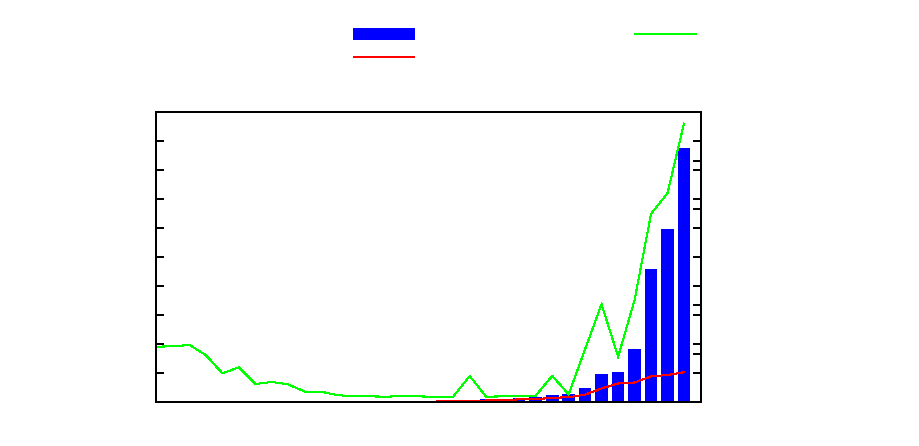
\includegraphics{DBs_comparison2}}%
    \gplfronttext
  \end{picture}%
\endgroup

	%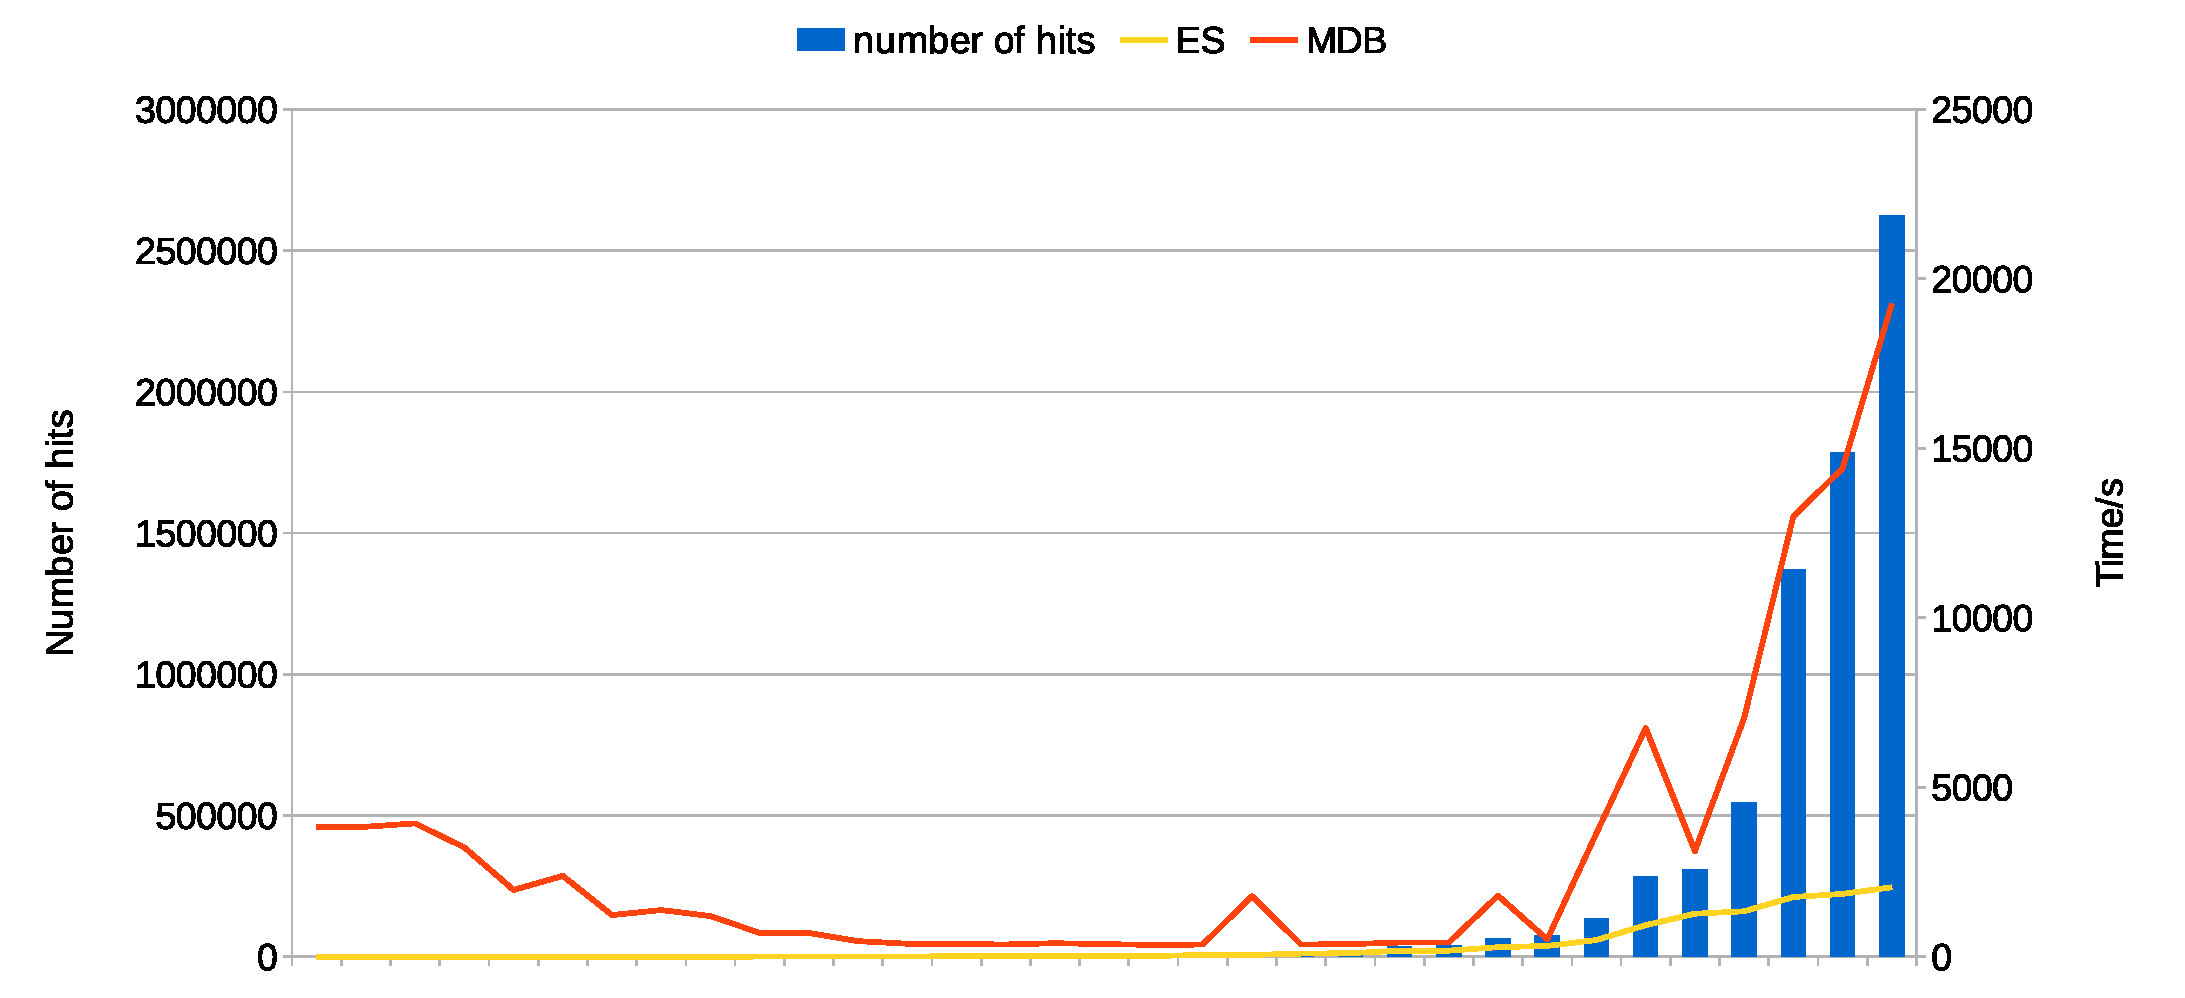
\includegraphics[width=\textwidth]{DBs_comparison.pdf}
	\caption{Comparison between ES and the best performing MongoDB (MDB WT) configuration.}
	\label{fig:DBscomparison}
\end{figure}

The queries on MongoDB are taking much more time than on Elasticsearch. MongoDB provides
a tool for explaining query execution. This becomes very useful when trying to investigate efficiency problems
like this one. In the listing in Appendix~\ref{app:MDB}, one can see the output of the command for one of the 
sample queries. The query planner tries all the indices associated with one of the queried properties, then 
selects one and based on just this one performs the search. The search results are then filtered so that the 
returned 
fields satisfy the other conditions of the input query. To test the best possible performance, special compound 
indices were created for each query and the performance was tested using these indices. 

\begin{figure}[h]
	\centering
	% GNUPLOT: LaTeX picture with Postscript
\begingroup
  \makeatletter
  \providecommand\color[2][]{%
    \GenericError{(gnuplot) \space\space\space\@spaces}{%
      Package color not loaded in conjunction with
      terminal option `colourtext'%
    }{See the gnuplot documentation for explanation.%
    }{Either use 'blacktext' in gnuplot or load the package
      color.sty in LaTeX.}%
    \renewcommand\color[2][]{}%
  }%
  \providecommand\includegraphics[2][]{%
    \GenericError{(gnuplot) \space\space\space\@spaces}{%
      Package graphicx or graphics not loaded%
    }{See the gnuplot documentation for explanation.%
    }{The gnuplot epslatex terminal needs graphicx.sty or graphics.sty.}%
    \renewcommand\includegraphics[2][]{}%
  }%
  \providecommand\rotatebox[2]{#2}%
  \@ifundefined{ifGPcolor}{%
    \newif\ifGPcolor
    \GPcolortrue
  }{}%
  \@ifundefined{ifGPblacktext}{%
    \newif\ifGPblacktext
    \GPblacktextfalse
  }{}%
  % define a \g@addto@macro without @ in the name:
  \let\gplgaddtomacro\g@addto@macro
  % define empty templates for all commands taking text:
  \gdef\gplbacktext{}%
  \gdef\gplfronttext{}%
  \makeatother
  \ifGPblacktext
    % no textcolor at all
    \def\colorrgb#1{}%
    \def\colorgray#1{}%
  \else
    % gray or color?
    \ifGPcolor
      \def\colorrgb#1{\color[rgb]{#1}}%
      \def\colorgray#1{\color[gray]{#1}}%
      \expandafter\def\csname LTw\endcsname{\color{white}}%
      \expandafter\def\csname LTb\endcsname{\color{black}}%
      \expandafter\def\csname LTa\endcsname{\color{black}}%
      \expandafter\def\csname LT0\endcsname{\color[rgb]{1,0,0}}%
      \expandafter\def\csname LT1\endcsname{\color[rgb]{0,1,0}}%
      \expandafter\def\csname LT2\endcsname{\color[rgb]{0,0,1}}%
      \expandafter\def\csname LT3\endcsname{\color[rgb]{1,0,1}}%
      \expandafter\def\csname LT4\endcsname{\color[rgb]{0,1,1}}%
      \expandafter\def\csname LT5\endcsname{\color[rgb]{1,1,0}}%
      \expandafter\def\csname LT6\endcsname{\color[rgb]{0,0,0}}%
      \expandafter\def\csname LT7\endcsname{\color[rgb]{1,0.3,0}}%
      \expandafter\def\csname LT8\endcsname{\color[rgb]{0.5,0.5,0.5}}%
    \else
      % gray
      \def\colorrgb#1{\color{black}}%
      \def\colorgray#1{\color[gray]{#1}}%
      \expandafter\def\csname LTw\endcsname{\color{white}}%
      \expandafter\def\csname LTb\endcsname{\color{black}}%
      \expandafter\def\csname LTa\endcsname{\color{black}}%
      \expandafter\def\csname LT0\endcsname{\color{black}}%
      \expandafter\def\csname LT1\endcsname{\color{black}}%
      \expandafter\def\csname LT2\endcsname{\color{black}}%
      \expandafter\def\csname LT3\endcsname{\color{black}}%
      \expandafter\def\csname LT4\endcsname{\color{black}}%
      \expandafter\def\csname LT5\endcsname{\color{black}}%
      \expandafter\def\csname LT6\endcsname{\color{black}}%
      \expandafter\def\csname LT7\endcsname{\color{black}}%
      \expandafter\def\csname LT8\endcsname{\color{black}}%
    \fi
  \fi
  \setlength{\unitlength}{0.0500bp}%
  \begin{picture}(8502.00,3968.00)%
    \gplgaddtomacro\gplbacktext{%
      \csname LTb\endcsname%
      \put(1342,264){\makebox(0,0)[r]{\strut{} 0.01}}%
      \put(1342,661){\makebox(0,0)[r]{\strut{} 0.1}}%
      \put(1342,1058){\makebox(0,0)[r]{\strut{} 1}}%
      \put(1342,1455){\makebox(0,0)[r]{\strut{} 10}}%
      \put(1342,1852){\makebox(0,0)[r]{\strut{} 100}}%
      \put(1342,2249){\makebox(0,0)[r]{\strut{} 1000}}%
      \put(1342,2646){\makebox(0,0)[r]{\strut{} 10000}}%
      \put(1342,3043){\makebox(0,0)[r]{\strut{} 100000}}%
      \put(6829,264){\makebox(0,0)[l]{\strut{} 1}}%
      \put(6829,661){\makebox(0,0)[l]{\strut{} 10}}%
      \put(6829,1058){\makebox(0,0)[l]{\strut{} 100}}%
      \put(6829,1455){\makebox(0,0)[l]{\strut{} 1000}}%
      \put(6829,1852){\makebox(0,0)[l]{\strut{} 10000}}%
      \put(6829,2249){\makebox(0,0)[l]{\strut{} 100000}}%
      \put(6829,2646){\makebox(0,0)[l]{\strut{} 1e+06}}%
      \put(6829,3043){\makebox(0,0)[l]{\strut{} 1e+07}}%
      \put(176,1653){\rotatebox{-270}{\makebox(0,0){\strut{}time(s)}}}%
      \put(7994,1653){\rotatebox{-270}{\makebox(0,0){\strut{}number of hits}}}%
    }%
    \gplgaddtomacro\gplfronttext{%
      \csname LTb\endcsname%
      \put(3230,3795){\makebox(0,0)[r]{\strut{}number of hits}}%
      \csname LTb\endcsname%
      \put(3230,3575){\makebox(0,0)[r]{\strut{}ES}}%
      \csname LTb\endcsname%
      \put(5933,3795){\makebox(0,0)[r]{\strut{}MDB WT}}%
      \csname LTb\endcsname%
      \put(5933,3575){\makebox(0,0)[r]{\strut{}MDB WT comp}}%
    }%
    \gplbacktext
    \put(0,0){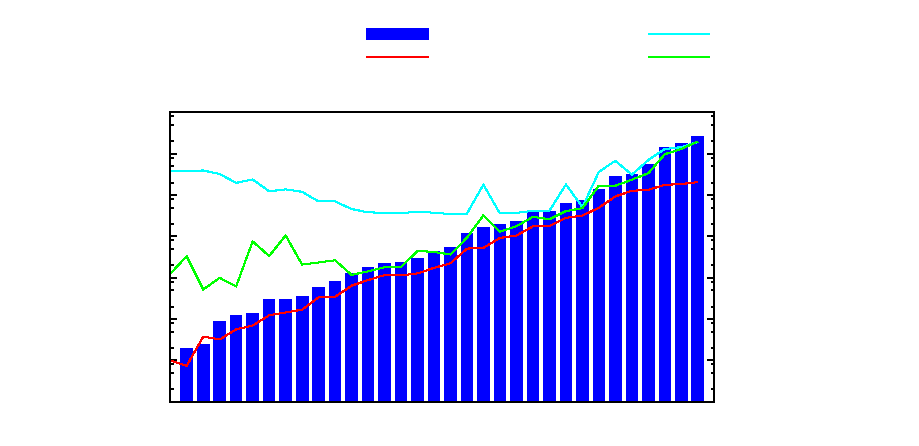
\includegraphics{MDBcompound}}%
    \gplfronttext
  \end{picture}%
\endgroup

	\caption{Comparison between MongoDB with indices created especially for the tested queries (MDB comp) and 
	ES. To show the improvement the MongoDB performance without the compound indices is graphed as well
	(MDB WT)}
	\label{fig:MDBcompound}
\end{figure}

Creating an index for each query is not the preferred usage pattern in this case. Also Figure~\ref{fig:MDBcompound} 
clearly states that even with these specialized indices MongoDB shows worse performance 
than Elasticsearch, although there is a great improvement when compared to the version without the new indices.  

\subsection{The Comparison Between NoSQL and the Current Deployment}

As we mentioned, currently the database back-end to all the services in DIRAC, where a database is needed including the File 
Catalog and its metadata part, is relying on MySQL. The table scheme of the metadata part of the DFC can be seen 
in Figure~\ref{fig:DFCUML}.

\begin{figure}[h]
	\centering
	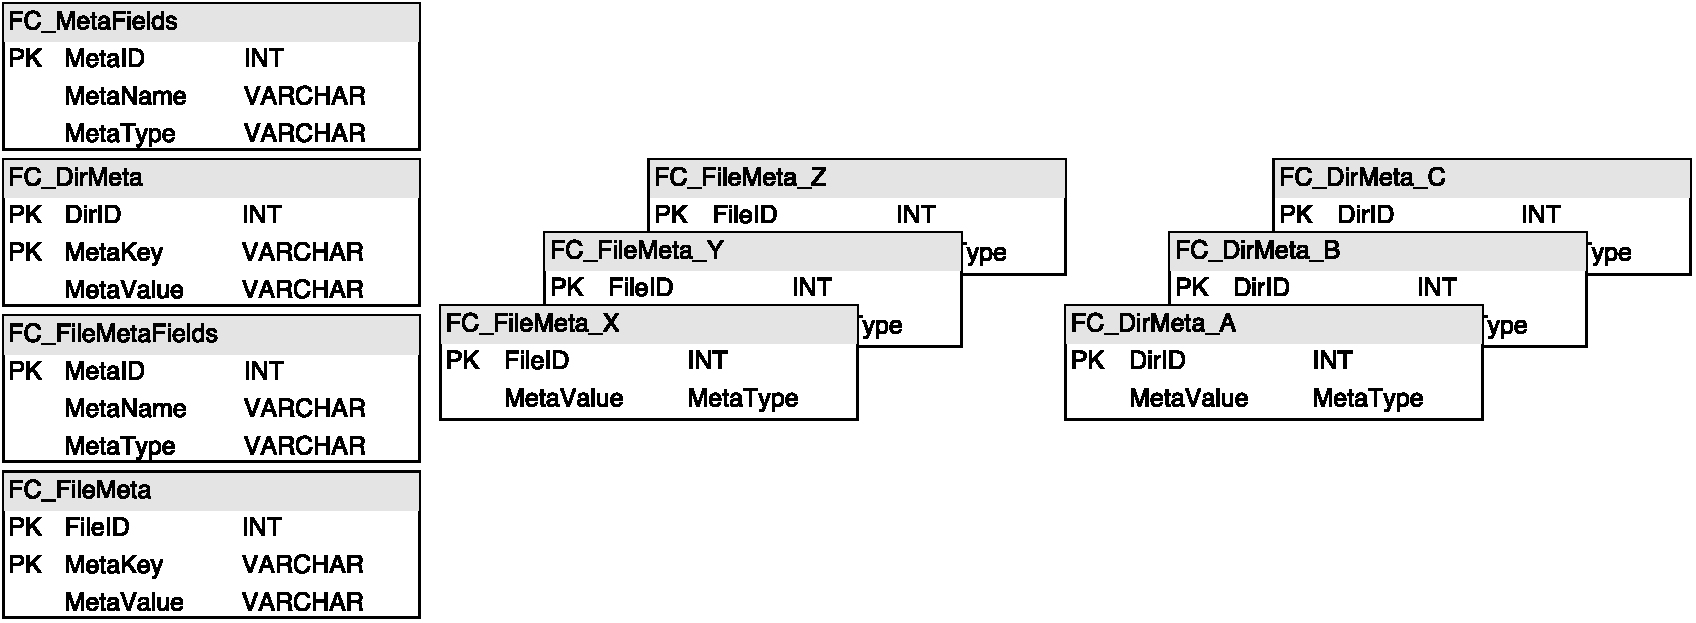
\includegraphics[width=\textwidth]{DFCDB.pdf}
	\caption{The File Catalog part of the database scheme. The tables on the left are created implicitly with the
	rest of the scheme. They are used  for keeping the track of the types of metafields and un-indexed  metadata 
	values. For each new indexed field a new table is created, in this scheme there are 3 indexed file metafields
	(X, Y, Z) and three indexed directory metafields (A,B,C).}
	\label{fig:DFCUML}
\end{figure}

In order to see if it is worth to start using a NoSQL database, in this project we compared the current deployment  
with the database that performed the
best in the tests we completed. When trying to test the MySQL database against the same queries 
by only loading the relevant data (creating tables only for 8 integer typed metadata and 3 string ones), the 
performance was much better than all the NoSQL databases. This was due to the fact, that the MySQL engine loaded
the whole dataset in memory and did not have to use the disk when executing the query. This however is not the expected 
behavior, because the database engine will most likely not serve only the DFC metadata catalog, so there will not
be enough memory space to keep all the metadata in cache. To test how the database could behave in production, the 
command \texttt{flush tables;} was used after every query to dump the cached tables. Also the whole dataset
was inserted into the database. This also let us to compare the size of data indexed by MySQL and by NoSQL (Table~\ref{tab:allDbSizes}). 

\begin{table}[t]
\centering
\begin{tabular}{lcc}
\toprule
\textbf{Database}      & & \textbf{Total database size}  \\ 
\midrule
MongoDB                & & 42 249                        \\ 
Elasticsearch          & & 59 715                        \\ 
csv files              & & 113 384                       \\ 
MySQL                  & & 185 135                       \\ 
\toprule
\end{tabular}
\caption{The comparison of disk usage for all databases. For an illustration the size of the input CSV files is
shown. All sizes are in MB.}
\label{tab:allDbSizes}
\end{table}

To test the databases more thoroughly a new set of queries was created. These queries involve more than just the 
small set of metafields indexed by the MongoDB. MySQL on this set proved itself better on queries consulting
a lesser number of metafields and a larger number of hits. Performance of Elasticsearch seems to correspond
to the number of hits while the complexity of the query does not seem to have an effect on its speed (results are provided 
in Figure~\ref{fig:wide}).

In all the tests above Elasticsearch and its indices were left with the default settings. Since ES is primarily 
a distributed store, the default setting assumes that there will be more than just one server in the cluster. This
means that for every read several nodes have to be contacted and even though the testing deployment consists of 
only one server, the index cut the data into 5 shards\footnote{A shard is a single Lucene instance. It is a low-level
``worker" unit which is managed automatically by Elasticsearch. An index is a logical namespace which points 
to primary and replica shards.} (default setting). The volume of data used 
in this project is not as large to need a whole cluster to be stored so it was re-indexed into an index 
with no replicas and only one primary shard, which is ideal when only one server is used. Also it comes closer to 
the MySQL database, because it can be run on only one server. The performance on re-indexed data was not 
significantly better and an even worse performance drop is observable when fetching a large number of documents. 
The queries contained from 2 to 6 conditions (consulted 2 to 6 different metadata).

\begin{figure}[h]
	\centering
	% GNUPLOT: LaTeX picture with Postscript
\begingroup
  \makeatletter
  \providecommand\color[2][]{%
    \GenericError{(gnuplot) \space\space\space\@spaces}{%
      Package color not loaded in conjunction with
      terminal option `colourtext'%
    }{See the gnuplot documentation for explanation.%
    }{Either use 'blacktext' in gnuplot or load the package
      color.sty in LaTeX.}%
    \renewcommand\color[2][]{}%
  }%
  \providecommand\includegraphics[2][]{%
    \GenericError{(gnuplot) \space\space\space\@spaces}{%
      Package graphicx or graphics not loaded%
    }{See the gnuplot documentation for explanation.%
    }{The gnuplot epslatex terminal needs graphicx.sty or graphics.sty.}%
    \renewcommand\includegraphics[2][]{}%
  }%
  \providecommand\rotatebox[2]{#2}%
  \@ifundefined{ifGPcolor}{%
    \newif\ifGPcolor
    \GPcolortrue
  }{}%
  \@ifundefined{ifGPblacktext}{%
    \newif\ifGPblacktext
    \GPblacktextfalse
  }{}%
  % define a \g@addto@macro without @ in the name:
  \let\gplgaddtomacro\g@addto@macro
  % define empty templates for all commands taking text:
  \gdef\gplbacktext{}%
  \gdef\gplfronttext{}%
  \makeatother
  \ifGPblacktext
    % no textcolor at all
    \def\colorrgb#1{}%
    \def\colorgray#1{}%
  \else
    % gray or color?
    \ifGPcolor
      \def\colorrgb#1{\color[rgb]{#1}}%
      \def\colorgray#1{\color[gray]{#1}}%
      \expandafter\def\csname LTw\endcsname{\color{white}}%
      \expandafter\def\csname LTb\endcsname{\color{black}}%
      \expandafter\def\csname LTa\endcsname{\color{black}}%
      \expandafter\def\csname LT0\endcsname{\color[rgb]{1,0,0}}%
      \expandafter\def\csname LT1\endcsname{\color[rgb]{0,1,0}}%
      \expandafter\def\csname LT2\endcsname{\color[rgb]{0,0,1}}%
      \expandafter\def\csname LT3\endcsname{\color[rgb]{1,0,1}}%
      \expandafter\def\csname LT4\endcsname{\color[rgb]{0,1,1}}%
      \expandafter\def\csname LT5\endcsname{\color[rgb]{1,1,0}}%
      \expandafter\def\csname LT6\endcsname{\color[rgb]{0,0,0}}%
      \expandafter\def\csname LT7\endcsname{\color[rgb]{1,0.3,0}}%
      \expandafter\def\csname LT8\endcsname{\color[rgb]{0.5,0.5,0.5}}%
    \else
      % gray
      \def\colorrgb#1{\color{black}}%
      \def\colorgray#1{\color[gray]{#1}}%
      \expandafter\def\csname LTw\endcsname{\color{white}}%
      \expandafter\def\csname LTb\endcsname{\color{black}}%
      \expandafter\def\csname LTa\endcsname{\color{black}}%
      \expandafter\def\csname LT0\endcsname{\color{black}}%
      \expandafter\def\csname LT1\endcsname{\color{black}}%
      \expandafter\def\csname LT2\endcsname{\color{black}}%
      \expandafter\def\csname LT3\endcsname{\color{black}}%
      \expandafter\def\csname LT4\endcsname{\color{black}}%
      \expandafter\def\csname LT5\endcsname{\color{black}}%
      \expandafter\def\csname LT6\endcsname{\color{black}}%
      \expandafter\def\csname LT7\endcsname{\color{black}}%
      \expandafter\def\csname LT8\endcsname{\color{black}}%
    \fi
  \fi
  \setlength{\unitlength}{0.0500bp}%
  \begin{picture}(8502.00,3968.00)%
    \gplgaddtomacro\gplbacktext{%
      \csname LTb\endcsname%
      \put(1210,440){\makebox(0,0)[r]{\strut{} 0.01}}%
      \put(1210,874){\makebox(0,0)[r]{\strut{} 0.1}}%
      \put(1210,1308){\makebox(0,0)[r]{\strut{} 1}}%
      \put(1210,1741){\makebox(0,0)[r]{\strut{} 10}}%
      \put(1210,2175){\makebox(0,0)[r]{\strut{} 100}}%
      \put(1210,2609){\makebox(0,0)[r]{\strut{} 1000}}%
      \put(1210,3043){\makebox(0,0)[r]{\strut{} 10000}}%
      \put(1342,220){\makebox(0,0){\strut{} 0}}%
      \put(2413,220){\makebox(0,0){\strut{} 10}}%
      \put(3484,220){\makebox(0,0){\strut{} 20}}%
      \put(4555,220){\makebox(0,0){\strut{} 30}}%
      \put(5626,220){\makebox(0,0){\strut{} 40}}%
      \put(6697,220){\makebox(0,0){\strut{} 50}}%
      \put(6829,440){\makebox(0,0)[l]{\strut{} 1}}%
      \put(6829,812){\makebox(0,0)[l]{\strut{} 10}}%
      \put(6829,1184){\makebox(0,0)[l]{\strut{} 100}}%
      \put(6829,1556){\makebox(0,0)[l]{\strut{} 1000}}%
      \put(6829,1927){\makebox(0,0)[l]{\strut{} 10000}}%
      \put(6829,2299){\makebox(0,0)[l]{\strut{} 100000}}%
      \put(6829,2671){\makebox(0,0)[l]{\strut{} 1e+06}}%
      \put(6829,3043){\makebox(0,0)[l]{\strut{} 1e+07}}%
      \put(176,1741){\rotatebox{-270}{\makebox(0,0){\strut{}time(s)}}}%
      \put(7994,1741){\rotatebox{-270}{\makebox(0,0){\strut{}number of hits}}}%
    }%
    \gplgaddtomacro\gplfronttext{%
      \csname LTb\endcsname%
      \put(3164,3795){\makebox(0,0)[r]{\strut{}Number of hits}}%
      \csname LTb\endcsname%
      \put(3164,3575){\makebox(0,0)[r]{\strut{}ES}}%
      \csname LTb\endcsname%
      \put(5867,3795){\makebox(0,0)[r]{\strut{}MySQL}}%
    }%
    \gplbacktext
    \put(0,0){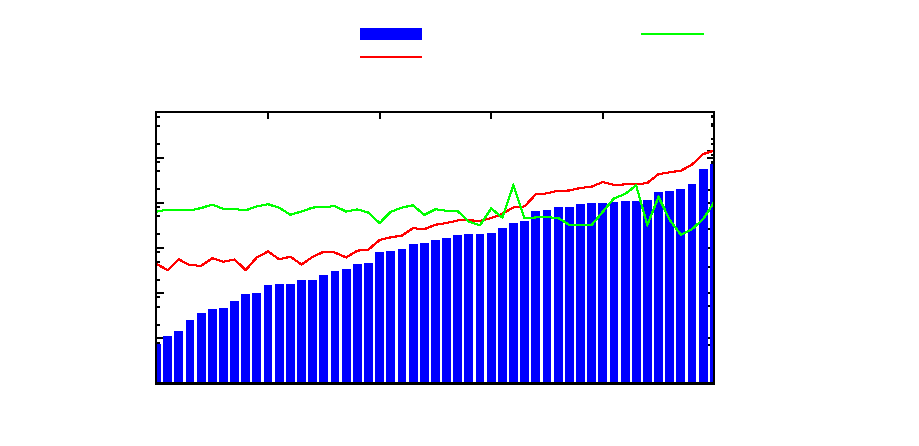
\includegraphics{ES_MySQL_wide}}%
    \gplfronttext
  \end{picture}%
\endgroup

	\caption{Comparison between the currently deployed MySQL and ES on a larger set of queries. 
	ES performance with data re-indexed to one shard is also graphed (ES one shard).}
	\label{fig:wide}
\end{figure}